\subsection{Architekturparadigmen}

In den Verteilten Systemen gibt es verschiedene Architekturparadigmen, die beschreiben, wie Software- oder Computersysteme strukturiert und organisiert werden können. Zunächst soll ein Überblick gegeben werden, bevor die Ansätze genauer diskutiert werden. Die wichtigsten Architekturparadigmen für diese Ausarbeitung sind:
\begin{itemize}  
\item \textbf{Schichtenarchitektur} (Layered Architecture): Hierbei wird das System in mehrere Schichten unterteilt, wobei jede Schicht eine bestimmte Funktion erfüllt und auf der darunter liegenden Schicht aufbaut. Ein Beispiel ist die dreischichtige Architektur, die aus einer Präsentationsschicht, einer Anwendungsschicht und einer Datenspeicherschicht besteht.

\item \textbf{Client-Server-Architektur}: Hierbei wird das System in einen Client und einen Server unterteilt, wobei der Client Anfragen an den Server sendet und dieser daraufhin Antworten liefert. Diese Architektur eignet sich gut für Anwendungen, bei denen der Client nur eine begrenzte Anzahl von Funktionen benötigt, während der Server die komplexen Berechnungen durchführt.

\item \textbf{Service-Orientierte Architektur} (SOA): Hierbei wird das System in Services unterteilt, die unabhängig voneinander entwickelt und bereitgestellt werden können. Diese Architektur ermöglicht die flexible Integration von Services, um komplexe Anwendungen zu erstellen.

\item \textbf{Ereignisgesteuerte Architektur} (Event-Driven Architecture): Hierbei reagiert das System auf Ereignisse, indem es entsprechende Aktionen ausführt. Diese Architektur wird oft in Systemen verwendet, die auf (beinah) Echtzeitereignisse reagieren müssen, wie z.B. in der Finanzindustrie oder in der Telekommunikation.

\item \textbf{Microservices-Architektur}: Hierbei wird das System in kleine, unabhängige Services unterteilt, die jeweils eine spezifische Funktion erfüllen. Diese Architektur ermöglicht eine bessere Skalierbarkeit und Flexibilität, da jeder Service unabhängig voneinander entwickelt, getestet und bereitgestellt werden kann.

\item \textbf{Peer-to-Peer-Architektur} (P2P): Hierbei wird das System in ein Netzwerk von gleichwertigen Teilnehmern unterteilt, die direkt miteinander kommunizieren können, ohne auf einen zentralen Server angewiesen zu sein. Diese Architektur wird oft in Filesharing- und Kryptowährungsanwendungen verwendet.
\end{itemize}  
Um Architekturmuster zu verstehen ist es auch wichtig zu hinterfragen, wie die Komponenten und Rechneneinheiten in einem System angeordnet sind. Um diese zu benennen wird häufig der Begriff \enquote{node}~\cite{tanenbaum2017distributed}~(Knoten) eingeführt. \textbf{Mit einem node versteht man ein autonomes Computerelement}, sei es Hardware-Systeme oder Software-Prozesse. 
Es gibt noch weitere Architekturparadigmen, aber diese sechs sind die in diesem Skript wichtigsten und am häufigsten verwendeten. Bei allen Architekturen darf man die historsche Komponente nicht vergessen. Die meisten Architekturen lassen sich daher auch aus dem Grundtypos einer Schichtenarchitektur erklären. 

\subsubsection{Schichtenarchitektur}

Schichtenmodelle spielen eine wichtige Rolle bei der Architektur von verteilten Systemen, indem sie hierarchische Strukturen definieren, die bestimmte Funktionen und Dienste je Schicht kapseln.
\\\\
Das Schichtenmodell ist ein durchdachtes Konzept, das auf dem Prinzip von \enquote{Teile und Herrsche} basiert und ein System in mehrere Ebenen unterteilt. Die Bedeutung von Schichtenmodelle für die Architektur von verteilten Systemen besteht darin, dass sie es ermöglichen, komplexe Systeme in kleinere, einfachere Teile zu zerlegen, die unabhängig voneinander entwickelt, getestet und gewartet werden können. Jede Schicht kann als eine separate Komponente oder ein separates Subsystem implementiert werden, das von anderen Schichten isoliert ist und über definierte Schnittstellen kommunizieren kann. Die besondere Bedeutung der Schnittstellen kann für den langfristen Erfolg nicht stark genug herausgestellt werden.

Durch die Verwendung von Schichtenmodellen wird auch die Interoperabilität zwischen verschiedenen Systemen erleichtert, da jeder Hersteller oder Entwickler eine bestimmte Schicht des Modells implementieren und somit sicherstellen kann. So ist das System im besten Falle mit anderen Systemen über die definierten Schnittstellen kompatibel.

Ein weiterer Vorteil bei der Verwendung der Architektur besteht darin, dass sie die Wiederverwendbarkeit von Komponenten und Diensten erleichtert. Da jede Schicht bestimmte Funktionen und Dienste bereitstellt, können sie in verschiedenen Systemen und Anwendungen wiederverwendet werden, ohne dass eine Neuentwicklung erforderlich ist. Schichten können auch dazu beitragen, die Sicherheit von Anwendungen zu verbessern. Durch die Trennung von Funktionen und Verantwortlichkeiten kann die Sicherheit jeder Schicht verbessert werden, ohne dass die Sicherheit des gesamten Systems beeinträchtigt wird. So kann beispielsweise eine Schicht, die für die Authentifizierung und Autorisierung von Benutzern verantwortlich ist, unabhängig von anderen implementiert und gewartet werden, um eine höhere Sicherheit zu gewährleisten.

Die Idee der Schichtenmodelle für verteilte Systeme geht auf die 1970er Jahre zurück, als verschiedene Organisationen begannen, Netzwerkprotokolle zu standardisieren und zu entwickeln. Das erste bekannte Schichtenmodell für Netzwerkprotokolle war das "Department of Defense (DoD) Internet Model", das 1982 von der US-amerikanischen Regierung eingeführt wurde. Dieses Modell hatte vier Schichten: Anwendung, Transport, Internet und Netzwerkzugang.

In den 1980er Jahren wurde das Open Systems Interconnection (OSI)-Referenz-modell von der Internationalen Organisation für Normung (ISO) eingeführt. Es war ein sehr generisches Schichtenmodell für Netzwerkprotokolle und hatte sieben Schichten: Anwendung, Darstellung, Sitzung, Transport, Netzwerk, Data Link und Physikalisch. Das OSI-Modell hatte den Vorteil, dass es herstellerunabhängig war und Interoperabilität zwischen verschiedenen Netzwerkprotokollen als definiertes Ziel umsetzte.

Auch andere Organisationen begannen ihre eigenen Schichtenmodelle für Netzwerkprotokolle zu entwickeln. Zum Beispiel verwendete die Digital Equipment Corporation (DEC) ein Schichtenmodell mit fünf Schichten, das DECnet genannt wurde. IBM entwickelte auch ein eigenes, das Systems Network Architecture (SNA) hieß.

In den 1990er Jahren gewannen TCP/IP-basierte Netzwerkprotokolle zunehmend an Bedeutung, und das OSI-Referenzmodell wurde weniger populär. TCP/IP hatte auch ein Schichtenmodell, das dem DoD Modell sehr ähnlich war. 
\\\\
In den letzten Jahren haben Schichtenmodelle auch bei der Entwicklung von verteilten Systemen jenseits von Netzwerken an Bedeutung gewonnen. Auch wenn das Modell manchmal recht angestaubt erscheint, wird es zum Beispiel verwendet, um die Architektur von Cloud-basierten Anwendungen oder Microservices zu beschreiben.
\\\\
Um die Kraft eines Schichtenmodells zu verdeutlichen, soll auch nochmal diskutiert werden, nach welchen Ansätzen ein System in Schichten unterschieden werden kann. Doch hierzu soll weniger der deutsche Begriff Schicht genutzt sein, sondern vielmehr  die englischen Begriffe \enquote{Tier} (Ebene) und \enquote{Layer} (Schicht). Diese Begriffe sind in dem Kontext gut etabliert und besser geeignet, um die notwendige Diskussion zu führen:
\\\\
Ein (Software-)\enquote{Layer} beschreibt eine logische Gruppierung von Funktionen innerhalb einer Anwendung oder eines Systems. Layer werden in der Regel vertikal angeordnet und können aus mehreren Tiers bestehen, die gemeinsam eine Schicht bilden. Jedes Layer erfüllt eine spezifische Funktion und  kommuniziert über definierte Schnittstellen mit der darüber oder darunter liegenden Schicht. Beispiele für Layer in verteilten Systemen sind die Three-Layer Architekturen, die in Anwendungslogik-Schicht, die Datenzugriffs-Schicht oder die Präsentations-Schicht unterteilt sind.
\begin{figure}[!h]
  \centering
  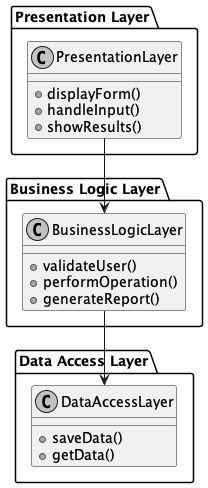
\includegraphics[width=0.25 \textwidth]{fig/uml/simple-layers.png}
  \caption{Einfaches Schichtenmodell}
  \label{fig:simple-layer}
\end{figure}

In dem Beispiel \ref{fig:simple-layer} sind drei Layer beschrieben, die jeweils eine Schicht darstellen:
\begin{itemize}
\item Das \enquote{Presentation Layer} enthält die Klasse "PresentationLayer", die für die Benutzeroberfläche und die Interaktion mit dem Benutzer zuständig ist.

\item Das \enquote{Business Logic Layer} enthält die Klasse "BusinessLogicLayer", die die Geschäftslogik und die Regeln enthält, die die Anwendung ausführen.

\item Das \enquote{Data Access Layer} enthält die Klasse \enquote{DataAccessLayer}, die für den Zugriff auf Datenbanken oder andere Datenquellen zuständig ist.
\end{itemize}
Die Pfeile zwischen den Komponenten zeigen die Abhängigkeiten zwischen den Schichten an. Die Presentation Layer ist von der Business Logic Layer abhängig und die Business Logic von der Data Access.
\\\\
Ein \enquote{Tier} hingegen beschreibt die physische oder logische Aufteilung von Anwendungen oder Systemen auf verschiedene Server oder Endgeräte. Jedes Tier hat normalerweise eine spezifische Funktion, wie z.B. Datenbank-Tier, Anwendungs-Tier oder Präsentations-Tier. Die Tiers sind normalerweise durch eine Netzwerkverbindung miteinander verbunden, und jede Schicht kommuniziert direkt mit jeder benachbarten Schicht.
\begin{figure}[!h]
  \centering
  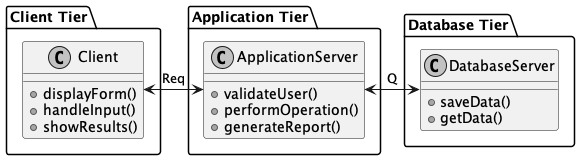
\includegraphics[width=0.80\textwidth]{fig/uml/simple-tiers.png}
  \caption{Einfaches Tier Modell}
  \label{fig:simple-tier}
\end{figure}
In diesem Beispiel eines Three-Tier-Models existieren drei Komponenten, die jeweils ein Tier darstellen:
\begin{itemize}
\item Das \enquote{Client Tier} enthält die Klasse \enquote{Client}, die für die Benutzeroberfläche und die Interaktion mit dem Benutzer auf dem Client-Gerät zuständig ist.

\item Das \enquote{Application Tier} enthält die Klasse \enquote{ApplicationServer}, die die Geschäftslogik und die Regeln enthält, die die Anwendung auf dem Application Server ausführen.

\item Das \enquote{Database Tier} enthält die Klasse \enquote{DatabaseServer}, die für den Zugriff auf Datenbanken oder andere Datenquellen auf dem Database Server zuständig ist.
\end{itemize}
Die Pfeile zwischen den Komponenten zeigen die Kommunikation zwischen den Tiers an. Der Client sendet eine Anfrage an den Application Server und der Application Server leitet die Anfrage an den Database Server weiter. Der Database Server gibt dann eine Antwort zurück, die über den Application Server an den Client zurückgesendet wird.
\\\\
Im Zweifel können Tiers und Layers die gleichen Namen besitzen, obwohl sich Ihre Motivation im Design unterscheidet. Vielleicht hilft auch nochmal die Sicht auf die Ziele der unterschiedlichen Zuschnitte. Im Layer-Modell sind folgende Ziele eher mit dem gewünschten Zuschnitt verbunden:
\begin{itemize}
\item Bestimmung der Funktionen und die Zuordnung zu logischen Komponenten mit fester Verantwortung und festen Schnittstellen. 
\item Bessere Wartbarkeit und die Flexibilität bei der Ausgestaltung. Komponenten können ausgetauscht und ersetzt werden, da sie festen Schnittstellendefinitionen genügen.  
\end{itemize}
Der Fokus auf die Tiers adressiert mehr die physischen Anforderung an die Architektur des verteilten Systems, diese sollen hier kurz nochmal erwähnt sein:
\begin{itemize}
\item Bestimmung der möglichen Skalierung auf (logische/virtuelle) Hardware und die generelle Zuweisung der logischen Komponenten.
\item Bestimmung der (Netzwerk-)Charakteristiken für die Kommunikation zwischen den Komponenten.
\end{itemize}
Ein besonderer Architekturtyp ist ein \enquote{Single-Node-Application}, welcher in einem Verteilten System als 1-Tier-Architektur verstanden werden kann.

\subsubsection{Single Node}

Eine Single-Node-Application ist ein Architekturtyp der das Ziel hat, das Anwendung auf einem einzelnen Knoten in einem verteilten System ausgeführt werden. Im Gegensatz zu einer Anwendung, die auf mehreren Knoten ausgeführt wird, braucht es hier keine Verteilung der Funktionen oder Daten über den logischen/physikalischen Knoten hinaus. Der Knoten kann ein physischer Server oder eine virtuelle Maschine sein.
\\\\
Ein Beispiel für eine Single-Node-Application in einem verteilten System könnte eine Anwendung sein, die Daten von verschiedenen Systemen sammelt und verarbeitet. Obwohl die Anwendung nur auf einem Knoten ausgeführt wird, muss sie möglicherweise mit verschiedenen Systemen und Datenquellen kommunizieren, dies ist in der Architektur nicht nur nicht ausgeschlossen, sondern eine erwünschte Eigenschaft.
\\\\
Obwohl Single-Node-Applications nicht auf mehreren Knoten verteilt sind, können sie immer noch von den Vorteilen einer Verteilung profitieren, wie z.B. Skalierbarkeit, Zuverlässigkeit und Flexibilität. Weiter können
Single-Node-Applications von Middleware-Technologien wie Message Queues und RPC profitieren, die die Interoperabilität zwischen verschiedenen Anwendungen und Systemen erleichtern. Eine Einschränkung ist, das die Middleware nicht primär für die kooperative Arbeit genutzt wird, sondern für das Sammeln und Aufbereiten der Daten. Diese Überlegungen münden in die Bestrebung der Formulierung eines Best Practice Entwurfmusters (Pattern) des sogenannten Single-Node-Pattern miteinfließen. Das Pattern hat seinen Nutzen bereits in verschiedenen Szenarien aufgezeigt, wie zum Beispiel:
\begin{itemize}
\item Entwicklung und Testen: Das Pattern kann verwendet werden, um Anwendungen auf einem einzigen Knoten während der Entwicklung und Tests auszuführen, um Zeit und Ressourcen zu sparen, die für die Bereitstellung und Verwaltung von verteilten Systemen erforderlich sind.
\item Kleine Anwendungen: Das Single-Node-Pattern kann nützlich sein, wenn die Anwendung klein ist und nicht viele Ressourcen benötigt. In diesem Fall kann eine entsprechende Implementierung ausreichend sein, um die Anforderungen der Anwendung zu erfüllen.
\item Datenintensive Anwendungen: Das Single-Node-Pattern ist auch für datenintensive Anwendungen nützlich, bei denen die Daten auf einem einzigen Knoten gespeichert und verarbeitet werden können.
\end{itemize}
Das Single-Node-Pattern kann mit verschiedenen Technologien implementiert werden, wie z.B. Container-Technologien (Docker), virtuelle Maschinen (VMs) oder Serverless-Computing (AWS Lambda). Die Wahl der Technologie hängt von den Anforderungen der Anwendung und den verfügbaren Ressourcen ab, welche Vor- und Nachteile verbunden sind, soll im Kapitel über die \enquote{Realisierung} miteinander diskutiert werden. 

\textbf{Das Single-Node-Pattern bezieht sich auf die Verwendung eines einzigen Serverknotens oder einer einzelnen Instanz des zu erbringenden Dienstes, anstatt mehrere Knoten zu verwenden, um denselben Dienst bereitzustellen}. Hier sind einige Beispiele von Unternehmen, die dieses Muster einsetzen:
\begin{itemize}
\item Netflix\footnote{https://medium.com/@narengowda/netflix-system-design-dbec30fede8d}: Netflix verwendet das Single-Node-Pattern, um die Datenverarbeitung in ihren AWS-Cloud-Instanzen zu optimieren. Sie haben sich dafür entschieden, ihre Anwendungen in kleinere, spezialisierte Dienste aufzuteilen, die auf einzelnen Knoten ausgeführt werden. Dies ermöglicht es ihnen, schnell auf Anforderungen zu reagieren, ohne Ressourcen für überflüssige Knoten zu verschwenden.
\item Airbnb\footnote{https://enqueuezero.com/airbnb-architecture.html}: Airbnb verwendet das Single-Node-Pattern, um ihre Webanwendung (Nicht die Daten) in einem einzigen Knoten zu hosten, anstatt sie auf mehrere Knoten aufzuteilen. Durch die Verwendung eines einzigen Knotens ist die Anwendung einfacher zu verwalten und zu skalieren. Airbnb kann schnell auf Veränderungen in der Nachfrage reagieren und ihre Anwendung schnell anpassen.
\end{itemize}

Für die weitere Diskussion müssen die physikalischen oder auch logischen Verbindungen zwischen Nodes diskutiert werden. Die logische Verbindung muss keiner physikalischen Verbindung entsprechen. Diese \enquote{virtuelle} Netzwerkstruktur besteht häufig auf der obersten Schicht einer physikalischen Netzwerkstruktur und wird als Overlay-Netzwerk bezeichnet. Ein Overlay-Netzwerk ermöglicht den Aufbau von Netzwerkdiensten und Anwendungen, die auf verteilten Systemen basieren, indem es zusätzliche Abstraktion und Organisation bietet. Das Ziel ist es, die Kommunikation und Zusammenarbeit zwischen den Knoten zu verbessern, die Skalierbarkeit zu erhöhen und die Netzwerkverwaltung zu vereinfachen. Sie ermöglichen es, verteilte Anwendungen und Dienste unabhängig von der zugrunde liegenden Netzwerkinfrastrukturen zu entwickeln und bereitzustellen. Allerdings können Overlay-Netzwerke auch zusätzliche Komplexität und Overhead verursachen, da sie auf bestehenden Netzwerkstrukturen aufbauen und von diesen abstrahiert sind, daher neigen Entwickler gerne dazu die bereits beschriebenen Fettnäpfchen zu suchen.

Ein Beispiel für ein Overlay-Netzwerk ist das Peer-to-Peer (P2P)-Overlay-Netzwerk~\cite{tanenbaum2017distributed}. In einem P2P-Netzwerk sind die Knoten gleichberechtigte Teilnehmer, die \textbf{direkt} miteinander kommunizieren und Ressourcen wie Rechenleistung, Speicherplatz und Bandbreite teilen. P2P-Netzwerke werden häufig für den Austausch von Dateien, die Verteilung von Inhalten oder die Bereitstellung von Streaming-Diensten verwendet.
\\\\
Ein bekanntes Beispiel für ein P2P-Overlay-Netzwerk ist das BitTorrent-Protokoll. BitTorrent ermöglicht den verteilten Austausch von Dateien über das Internet, indem es die Dateien in kleinere Teile (sogenannte Chunks) aufteilt und diese über mehrere Peers verteilt. Jeder Peer, der an einem Dateiaustausch teilnimmt, lädt Teile der Datei von anderen Peers herunter und stellt gleichzeitig bereits heruntergeladene Teile für andere Peers zur Verfügung. Auf diese Weise wird die Last auf die einzelnen Knoten im Netzwerk verteilt, und die Geschwindigkeit und Zuverlässigkeit des Dateiaustauschs verbessert.
\\\\
\textbf{Strukturierte} und \textbf{unstrukturierte} Netzwerke sind zwei verschiedene Ansätze für die Organisation und den Aufbau von verteilten Systemen bzw. Overlay-Netzwerken. Beide haben ihre eigenen Vor- und Nachteile, abhängig von den Anforderungen und dem Nutzungszweck des Netzwerks.
\begin{itemize} 
\item Organisation: Strukturierte Netzwerke sind durch eine gut definierte und geordnete Struktur gekennzeichnet. Sie verwenden meist deterministische Verfahren oder Algorithmen, um die Verbindungen zwischen den Knoten im Netzwerk herzustellen und aufrechtzuerhalten. Unstrukturierte Netzwerke haben keine festgelegte oder geordnete Struktur. Die Verbindungen zwischen den Knoten im Netzwerk werden zufällig oder auf der Grundlage von Heuristiken hergestellt. Dies beeinflusst die Art der Kommunikation und hat großen Einfluss auf die Algorithmen die anwendbar sind. Dies wird in dem Kapitel über die Algorithmen nochmal gesondert diskutiert.
\item Routing: Das Routing in strukturierten Netzwerken ist effizienter und vorhersagbarer, da es auf der Grundlage der Netzwerkstruktur erfolgt. Erfahrungen können auch in Lehrmodulen wie Rechnernetze im Kontext von IP Netzen gesammelt werden. Ein weiteres Beispiel für ein strukturiertes Routing-Verfahren ist das Distributed Hash Table (DHT), bei dem die Knoten und Ressourcen auf der Grundlage von Hash-Werten organisiert sind. Im Gegensatz zu strukturierten Netzwerken ist das Routing in unstrukturierten Netzwerken weniger effizient und vorhersagbar. Die Nachrichten können mehrere Hops zwischen Knoten benötigen, um ihr Ziel zu erreichen, und es kann zu einer höheren Netzwerkbelastung führen.
\item Suche: In strukturierten Netzwerken ist die Suche nach Ressourcen oder Knoten meist schneller, da sie auf vordefinierten Pfaden und Algorithmen basiert. Die Suche kann in logarithmischer Zeit (O(log N)) durchgeführt werden, wobei N die Anzahl der Knoten im Netzwerk ist, diese Optimierung bedarf aber einer weitergehende Baumstruktur. Die Suche in unstrukturierten Netzwerken erfolgt meist über Flooding- oder Random-Walk-Verfahren, bei denen eine Anfrage an mehrere Knoten gleichzeitig gesendet wird. Dies kann zu längeren Suchzeiten und höherer Netzwerkbelastung führen, insbesondere in großen Netzwerken. Auch diese beide Verfahren werden noch im weiteren Skript erläutert. 
\item Skalierbarkeit: Strukturierte Netzwerke sind im Allgemeinen besser skalierbar und eignen sich für große, verteilte Systeme, da die Organisation und das Routing effizienter gestaltet sind.
Unstrukturierte Netzwerke sind in der Regel weniger skalierbar als strukturierte Netzwerke, da sie anfälliger für Netzwerkengpässe und ineffizientes Routing sind. Sie eignen sich jedoch für kleinere Netzwerke oder Anwendungen, bei denen eine flexible und dynamische Organisation wichtiger ist als Effizienz.
\end{itemize} 
Aber nicht nur die Struktur stellt das Design vor unterschiedliche Herausforderungen, auch die Einordnung in bekannte und unbekannte Kommunikationspartner und wie man diese in Gruppen organisiert oder Ressourcen auch vor schädlichen Teilnehmern schützt.

\subsubsection{Middleware Architektur}
Neben dem Bedürfnis der Verteilung steht auch die Kapslung der Aufgabe für die Verteilung Fokus. So wäre es zielgerichtet, nach den bisherigen Diskussionen, eine Schicht zu kreieren, welche die Aufgaben der Verteilung in sich vereint.
\cite{tanenbaum2017distributed} beschreibt die Aufgaben einer solchen Schicht als Middleware mit:
\begin{itemize}
\item Bereitstellung eines breiten Angebotes für die \textbf{Kommunikation}: 
Eine wichtige Funktion der Middleware ist die Bereitstellung eines umfangreichen Satzes von Kommunikationsprotokollen, die die Interaktion zwischen verschiedenen Anwendungen und Systemen ermöglichen. Diese Protokolle stellen sicher, dass Daten zwischen verschiedenen Anwendungen und Systemen effizient und sicher ausgetauscht werden können. Wesentliche Vorarbeiten für diesen Bereich werden in einem Lehrmodul wie Rechnernetze angelegt.
\item Dem (Un\textbf{)Marshalling}\index{Marshalling} Prozess: Ein weiterer wichtiger Aspekt von Middleware ist das (Un)Marshalling von Daten, das für integrierte Systeme notwendig ist. (Un)Marshalling bezieht sich auf den Prozess des Konvertierens von Daten in ein Format, das von einer anderen Anwendung oder einem anderen System verwendet werden kann. Die Middleware bietet die notwendigen Mechanismen, um Daten zwischen verschiedenen Systemen in einem Format zu konvertieren, das von allen beteiligten Anwendungen und Systemen verstanden werden kann. Einzelne Beispiele für die Anforderungen werden auch in diesem Skript diskutiert. 
\item Protokolle zur \textbf{Namensauflösung}: Darüber hinaus bieten Middleware-Dienste auch Namensprotokolle, die es ermöglichen, Ressourcen einfach zu teilen. Mit Namensprotokollen können Ressourcen in einem verteilten System mit einem eindeutigen Namen identifiziert und von verschiedenen Anwendungen und Systemen einfach referenziert werden. Hier muss zunächst eine Diskussion über Identifier und Namen geführt werden, um die Möglichkeiten breit zu diskutieren. Dies geschieht im Kapitel Service-Discovery.
\item \textbf{Sicherheitsprotokolle}: Auch ist die Bereitstellung von Sicherheitsprotokollen ein wichtiges Merkmal. Diese Protokolle bieten Mechanismen zur Verschlüsselung von Daten und zur Authentifizierung von Benutzern und Systemen, um sicherzustellen, dass nur autorisierte Benutzer auf das System zugreifen können und dass Daten während der Übertragung verschlüsselt und gesichert sind. Sicherheit wird in diesem Skript nicht detaillierter diskutiert.
\item \textbf{Mechanismen zur} Steigerung der \textbf{Skalierung}: Schließlich bietet Middleware auch Skalierungsmechanismen wie Replikation und Caching, um die Leistung von Anwendungen in einem verteilten System zu verbessern. Diese Mechanismen ermöglichen die Duplizierung von Daten und Ressourcen auf verschiedenen Systemen, um die Verfügbarkeit und Zuverlässigkeit von Anwendungen zu erhöhen. Diese Punkte werden nochmals genauer in späteren Kapitel über die Realisierung diskutiert.
\end{itemize}
Ein großer Vorteil ist, das für den Applikationsentwickler nur die Entwicklung des Anwendungsprotokolls bleibt. Im besten Fall bietet die Schnittstelle der Middlewareschicht ein abstrahiertes \enquote{Interface}, welches sich im besten Fall nicht von einem Standalone System abgrenzen lässt, sich somit verhält wie ein kohärentes System. Das Interface, mit der verbundenen Realisierung hat das primäre Ziel Interoperabilität über verschiedene Systeme. Diese Aufgabe kann auch wieder in einzelne Aufgaben geteilt werden: 
\begin{itemize}
\item Mehrere Sprachen unterstützen: Middleware kann verwendet werden, um die Interoperabilität zwischen verschiedenen Anwendungen zu verbessern, die in verschiedenen Programmiersprachen geschrieben sind. Die Middleware kann als Übersetzungsschicht dienen, um Nachrichten zwischen den Anwendungen zu übersetzen und sicherzustellen, dass sie in der korrekten Syntax und Semantik gesendet und empfangen werden.
\item Mit mehreren Betriebssystemen und Hardwaretypen arbeiten: Eine Middleware kann dazu beitragen, die Interoperabilität zwischen Anwendungen zu verbessern, die auf verschiedenen Betriebssystemen und Hardwaretypen ausgeführt werden. Die Middleware kann als eine Abstraktionsschicht dienen, die es den Anwendungen ermöglicht, unabhängig von der zugrunde liegenden Hardware und dem Betriebssystem zu arbeiten.
\item Mehrere Netzwerkprotokolle unterstützen: Middleware kann verwendet werden, um die Interoperabilität zwischen Anwendungen zu verbessern, die verschiedene Netzwerkprotokolle verwenden. Die Middleware kann als eine Schicht dienen, die es den Anwendungen ermöglicht, Nachrichten in einem bestimmten Protokoll zu senden und zu empfangen, unabhängig davon, welches Protokoll von der anderen Anwendung verwendet wird.
\end{itemize}
Um die Kommunikation innerhalb eine Middleware-Schicht zu realisieren ergeben sich unterschiedliche Ansätze für die Kommunikation, die zuächst kurz eingeführt werden sollen. Wichtig für den Lernerfolg ist mitzunehmen, das diese Alternativen auch über die Middleware hinaus Gültigkeit haben.  
\begin{itemize}
\item \textbf{Point to point}\\
Die Point-to-Point-Kommunikation kann in einem verteilten System auf verschiedene Arten implementiert werden, wie zum Beispiel durch die Verwendung von Messaging-Systemen oder direkter Socket-Kommunikation. In beiden Fällen muss der Absender die Adresse des Empfängers kennen, um die Nachricht zu senden.
\\\\
Point-to-Point-Nachrichten werden häufig verwendet, um bestimmte Aufgaben oder Transaktionen zwischen verschiedenen Komponenten oder Diensten in einem verteilten System auszuführen. Zum Beispiel kann eine Anwendung eine Point-to-Point-Nachricht senden, um eine Anforderung an einen anderen Dienst im System zu stellen, um eine bestimmte Aktion auszuführen oder eine Antwort auf eine Anfrage zu erhalten. Vorteile von Point-to-Point-Nachrichten sind unter anderem:
\begin{itemize}
\item Effizienz: Sie sind selbst effizienter als Multicast/ Broadcast-Nachrichten, wenn sie auf einem Medium ausgeführt werden, welches primär dezidierte Kommunikation zwischen zwei Kommunikationspartner ermöglicht. Der Aufwand ist dann gering, da sie nur an einen spezifischen Empfänger gesendet werden, der die Nachricht empfangen soll. Im besten Fall ist nicht mal eine Adressierung notwendig. 
\item Präzision: Sie sind auf jeden Fall präziser als Broadcast-Nachrichten, da sie nur an den Empfänger gesendet werden, der die Nachricht empfangen soll, was das Risiko von Konflikten oder Fehlern verringert. So können sie auch für einen bestimmten Empfänger oder Sender optimiert werden.
\end{itemize} 
Wichtig an dem Beispiel in \ref{lst:p2p-message} ist, dass in diesem Fall die Middleware sich über die Nachricht bewusst sein muss. Es werden noch generischere Ansätze diskutiert werden, wo die Middleware keine Annahmen über die Nachricht selbst formuliert, dies ist beispielhaft bei RPC der Fall. 

Bei der Kodierung von Nachrichten können verschiedene Freiheitsgrade genutzt werden. Eine Auswahl von Beispielen sollen an dem Fallbeispiel der Lampe besprochen werden. Zur Steuerung einer Lampenschaltung gibt es verschiedene Möglichkeiten, je nach Komplexität der Anforderungen und der verwendeten Kommunikationstechnologie. Hier sind einige Beispiele für verschiedene Codierungsansätze:
\newpage
\begin{lstlisting}[caption={Message für Point to Point Kommunikation},captionpos=b,label={lst:p2p-message}]
{
   "message_id": "12345",
   "sender": "applicationA",
   "receiver": "applicationB",
   "payload": {
      "command": "update_customer",
      "customer_id": "67890",
      "data": {
         "first_name": "John",
         "last_name": "Doe",
         "email": "johndoe@example.com"
      }
   }
}
\end{lstlisting}

\begin{itemize}
\item Binäre Codierung (0 und 1): Die einfachste Form der Codierung besteht darin, die Lampe mit einem einzigen Binärwert über eine Point-to-Point Verbindung zu steuern. Eine logische \enquote{0} könnte \enquote{Lampe aus} bedeuten, während eine \enquote{1} \enquote{Lampe an} bedeutet. Dieser Ansatz ist sehr einfach und eignet sich für grundlegende Anwendungen.
\item Zeichenketten (Text): Eine andere Möglichkeit ist die Verwendung von Zeichenketten zur Codierung von Nachrichten. Zum Beispiel könnte die Nachricht \enquote{ON} verwendet werden, um die Lampe einzuschalten, und \enquote{OFF}, um sie auszuschalten. Dieser Ansatz ist etwas ausführlicher als die Binärcodierung, ermöglicht aber auch eine einfachere Interpretation und Erweiterbarkeit, wenn zusätzliche Funktionen hinzugefügt werden müssen.
\item Enumerations: Für eine klarere Struktur und Typsicherheit können Enumerations verwendet werden. Enums definieren einen Satz von benannten Werten, die die möglichen Zustände der Lampe darstellen. Zum Beispiel: \enquote{LAMPE\_AN} und \enquote{LAMPE\_AUS}. Dieser Ansatz ist gut lesbar und ermöglicht eine leichtere Erweiterung bei der Hinzufügung neuer Funktionen.
\item TLV\footnote{Typ Length Value} Strukturen: Für komplexere Anwendungen, in denen mehrere Attribute oder Parameter beteiligt sein können, können TLV-Strukturen verwendet werden. In einer TLV-Struktur wird jeder Parameter durch einen Typ, eine Länge und einen Wert dargestellt. Zum Beispiel könnte der Typ \enquote{1} für die Lampensteuerung verwendet werden, die Länge gibt die Anzahl der Bytes für den Wert an und der Wert selbst repräsentiert den gewünschten Zustand der Lampe (z. B. \enquote{0} für aus, \enquote{1} für an). TLV-Strukturen sind flexibel, erweiterbar und eignen sich gut für verteilte Systeme und komplexe Anwendungen. Tatsächlich kann eine TLV Struktur binär als String, aber auch mit JSON oder XML kodiert werden.
\end{itemize}

\item \textbf{Point to multipoint}: Eine Point-to-Multipoint Kommunikation zeichnet sich dadurch aus, dass eine Nachricht von einem Absender an mehrere Empfänger in einem verteilten System gesendet wird. 
\\\\
Ein Beispiel für eine Point-to-Multipoint-Nachricht wäre eine Nachricht, die an eine Gruppe von Abonnenten in einem Nachrichtenbroker-System gesendet wird. Der Absender sendet die Nachricht an den Broker, der die Nachricht dann an alle Abonnenten weiterleitet, die diese spezifische Nachricht abonniert haben.
\\\\
Ein anderes Beispiel wäre ein System zur Überwachung von Sensoren in einer Fabrik. Der Absender kann eine Point-to-Multipoint-Nachricht an alle Sensoren senden, um ein Update der Einstellungen oder einen Alarm zu senden, anstatt eine Point-to-Point-Nachricht an jeden Sensor einzeln zu senden.  Auch einer Point-to-Multipoint-Kommunikation kann man ähnliche Vorteile wie der Point-to-Point Kommunikation abgewinnen, nur mit anderen Vorzeichen:
\begin{itemize}
\item Effizienz: Point-to-Multipoint-Nachrichten sind effizienter als Point-to-Point-Nachrichten auf Übertragungsmedien die inhärent Boradcast sind bzw. Strukturen und Komponenten für diese Kommunikation vorsehen, da sie an mehrere Empfänger gleichzeitig gesendet werden können und somit die Netzwerklast reduzieren können.
\item Skalierbarkeit: Point-to-Multipoint-Nachrichten sind skalierbar und können in verteilten Systemen mit vielen Empfängern verwendet werden, solange das Medium die Übertragung entsprechend unterstützt.
\item Einfache Implementierung: Point-to-Multipoint-Nachrichten können einfach implementiert werden, da sie in vielen Messaging-Systemen und Protokollen unterstützt werden, was in einem einfachen Interface mündet auch wenn die Vorarbeiten komplex gestaltet sein können.
\item Schnellere Verarbeitung: Point-to-Multipoint-Nachrichten können schneller verarbeitet werden als Point-to-Point-Nachrichten, da sie im besten Fall nur einmal gesendet und an den Knoten nur einmalig weitergeltet werden müssen, anstatt an jeden Empfänger einzeln.
\end{itemize}
Point-to-Multipoint-Nachrichten sind ein wichtiger Bestandteil von verteilten Systemen und bieten insbesondere im Kontext der Replikation große Vorteile.
\item \textbf{Event/action}: Diese Art der Kommunikation beschreibt mehr den Mechanismus bei der Kommunikation. So kann man die notwendigen Elemente in 5 Punkte beschreiben:
\begin{itemize}
\item Ereignisquellen: Ereignisquellen sind Dienste oder Komponenten in einem verteilten System, die Ereignisse, den Event, erzeugen und an das System senden können. Diese Ereignisse können von verschiedenen Arten sein, z.B. Benutzeraktionen, Systemmeldungen oder Datenaktualisierungen.
\item Ereignisverarbeitung: Ereignisverarbeitung ist der Mechanismus, mit dem Ereignisse im verteilten System erfasst, verarbeitet und in einen Zustand umgewandelt werden, der für die weiteren Aktionen verwendet werden kann. Dies kann beinhalten, die Ereignisse zu filtern, zu transformieren oder zu aggregieren.
\item Ereignisrouting: Ereignisrouting ist der Mechanismus, mit dem Ereignisse an die richtigen Dienste oder Komponenten im verteilten System weitergeleitet werden. Dies kann durch die Verwendung von Routing-Regeln, Ereignisfiltern oder anderen Methoden erfolgen.
\item Ereignisempfang: Ereignisempfang ist der Mechanismus, mit dem Ereignisse von verschiedenen Quellen im verteilten System empfangen werden können. Dies kann durch die Verwendung von APIs, Messaging-Systemen oder anderen Methoden erfolgen.
\item Ereignisreaktion: Ereignisreaktion ist der Mechanismus, mit dem das System auf Ereignisse reagiert, die empfangen wurden. Dies kann die Ausführung von Aktionen, die Aktualisierung von Daten oder die Weiterleitung von Ereignissen an andere Komponenten oder Dienste beinhalten.
\end{itemize}
Wichtig ist in diesem Kontext zu verstehen, dass, obwohl die Kombination Event/Aktion sehr intuitiv erscheint, die dafür notwendigen Konstruktionen sehr aufwendig sein können. Insbesondere das Ereignisrouting kann eine hohe Komplexität einnehmen. 

\item \textbf{Publish/subscribe}: Publish/Subscribe ist ein Kommunikationsform, bei den Komponenten oder Dienste sich für bestimmte Ereignisse oder Nachrichten anmelden und dann automatisch benachrichtigt werden, wenn diese Ereignisse oder Nachrichten auftreten.

Das Muster besteht aus zwei Hauptkomponenten: dem Publisher\index{publisher} und dem Subscriber\index{subscriber}. Der Publisher ist für das Erzeugen und Senden von Ereignissen oder Nachrichten an das System verantwortlich. Der Subscriber ist für das Abonnieren von Ereignissen oder Nachrichten und für das Empfangen von Benachrichtigungen über diese Ereignisse oder Nachrichten verantwortlich. Das genutzte Publish/Subscribe-Pattern ermöglicht eine lose Kopplung zwischen dem Publisher und dem Subscriber. 

Der Publisher muss nicht wissen, wer die Ereignisse oder Nachrichten empfängt, und der Subscriber muss nicht wissen, woher die Ereignisse oder Nachrichten kommen. Dies ermöglicht eine höhere Flexibilität und Skalierbarkeit des Systems, da neue Komponenten oder Dienste einfach hinzugefügt oder entfernt werden können, ohne dass dies Auswirkungen auf andere Komponenten oder Dienste hat.

Das Muster kann auf verschiedene Arten implementiert werden, z.B. durch die Verwendung von Messaging-Systemen, die die Kommunikation zwischen dem Publisher und dem Subscriber verwalten, oder durch die Verwendung von APIs, die es dem Subscriber ermöglichen, Ereignisse oder Nachrichten direkt vom Publisher zu empfangen.
\\\\
Ein Beispiel für die Verwendung von Publish/Subscribe ist ein System zur Überwachung von Sensoren in einer Fabrik. Die Sensoren senden Ereignisse an das System, wenn sie ein Problem erkennen. Die verschiedenen Komponenten des Systems, wie z.B. das Alarmierungssystem oder das Wartungssystem, abonnieren diese Ereignisse und werden automatisch benachrichtigt, wenn ein Problem auftritt. Dadurch kann das System schnell auf Probleme reagieren und effizienter arbeiten.
\\\\
Wichtig wahrzunehmen ist, dass die Realisierung eines Publish/Subscribe meist selbst ein verteiltes System darstellt und meist über Point-to-Point kommuniziert, obwohl ein Point-to-Multipoint besser geeignet wäre.
\item \textbf{Client/Server}, Request/Reply\\
Neben dem später diskutierten Client/Server-Archtekturmuster, existiert auch das Client/Server Kommunikationsmuster. Das Client/Server-Kommunikations-muster ist ein grundlegendes Pattern in der Entwicklung von Netzwerkanwendungen, bei dem eine Anwendung (der Client) eine Verbindung zu einer anderen Anwendung (dem Server) herstellt, um eine bestimmte Aktion oder Dienstleistung anzufordern.
\\\\
In diesem Muster sendet der Client eine Anfrage an den Server, die eine bestimmte Aktion oder ein bestimmtes Ergebnis erfordert. Der Server verarbeitet die Anfrage und sendet eine Antwort zurück an den Client, die das Ergebnis der Anfrage enthält.
\\\\
Das Client/Server-Kommunikationsmuster ermöglicht es, komplexe Anwendungen aufzubauen, indem verschiedene Komponenten oder Dienste in einem verteilten System miteinander kommunizieren. Der Client kann verschiedene Anfragen an den Server senden, z.B. die Abfrage von Daten oder die Ausführung von Operationen, und der Server kann entsprechend antworten und die angeforderten Dienste bereitstellen.
\\\\
Das Muster kann auf verschiedene Arten implementiert werden, z.B. durch die Verwendung von APIs, die es dem Client ermöglichen, Anfragen direkt an den Server zu senden, oder durch die Verwendung von Messaging-Systemen, die die Kommunikation zwischen dem Client und dem Server verwalten.
\\\\
Ein Beispiel für die Verwendung des Client/Server-Kommunikationsmusters ist eine Webanwendung, bei der ein Benutzer eine Anfrage an einen Webserver sendet, um eine bestimmte Webseite anzuzeigen. Der Webserver verarbeitet die Anfrage und sendet die entsprechende Webseite an den Browser des Benutzers zurück.
\\\\
In diesem Fall wird sogar durch die Nutzung des HTTP Protokolls, das Request/Reply-Muster angewendet, welches eine spezielle Form der Client/Server-Kommunikation beschreibt. In diesem Fall wird immer in einer synchronen Kommunikation eine Anfrage (Request) gestellt und auf die Antwort (Reply/Response) gewartet. Andere Client/Server-Kommunikationsmuster können auch asynchron sein.
\\\\
Das Client/Server-Kommunikationsmuster ist eine effektive Möglichkeit, verteilte Anwendungen zu entwickeln, indem es eine einfache Methode zur Kommunikation zwischen verschiedenen Komponenten und Diensten bietet. Basis der Kommunikation kann eine Point-to-Point, Point-to-Multipoint aber auch Publish/Subscribe Kommunikations sein. 

\item \textbf{Mobile code}\\
Mobile Code ist ein Konzept in verteilten Systemen, bei dem ein Stück Code von einem Computer zu einem anderen Computer transportiert und auf diesem ausgeführt wird. Der Code wird dabei in der Regel als ausführbare Datei oder Skript über das Netzwerk übertragen.

Mobile Code ermöglicht es, Anwendungen und Dienste zu entwickeln, die auf verteilten Systemen ausgeführt werden können. Ein Beispiel für die Verwendung von Mobile Code ist die Remote-Ausführung von Skripten oder Programmen auf einem Server, der von einem Client-Computer aus gesteuert wird. Ein weiteres Beispiel ist die Verwendung von JavaScript in Webbrowsern, bei denen der Code von einer Website heruntergeladen und auf dem Client-Computer ausgeführt wird.

Ein aktuelles Beispiel für die Verwendung von Mobile Code ist die Verwendung von Container-Technologien wie Docker oder Kubernetes. Container können als mobile Code betrachtet werden, da sie Anwendungen und deren Abhängigkeiten in einem einzigen Paket bündeln und es ermöglichen, diese auf verschiedenen Computern und Betriebssystemen auszuführen. Container-Images können auf einem Server erstellt und dann auf andere Server oder Cloud-Plattformen verteilt werden, wo sie ausgeführt werden können.

Mobile Code birgt jedoch auch Risiken, da er Sicherheitsprobleme wie die Möglichkeit der Einschleusung von Malware oder Viren auf dem Zielcomputer aufgrund fehlender Kontrolle über den ausgeführten Code verursachen kann. Es ist wichtig, geeignete Sicherheitsmechanismen und Überprüfungsverfahren zu implementieren, um diese Risiken zu minimieren.

Für die Übertragung von Mobile Code braucht es wieder rudimentärere Kommunikationsmuster. s
\item \textbf{Virtual shared} \\
Virtual Shared Memory (VSM) ist ein Konzept in verteilten Systemen, dass es mehreren Prozessen ermöglicht, auf gemeinsamen Speicher zuzugreifen, als ob sie physisch auf demselben Computer ausgeführt würden. Dabei wird ein virtueller Adressraum bereitgestellt, der auf mehreren Computern verteilt ist, aber für die Prozesse so aussieht, als ob er auf einem einzigen Computer lokalisiert wäre.

Das VSM-Konzept ermöglicht es, die Kommunikation und den Datenaustausch zwischen verschiedenen Prozessen in einem verteilten System zu optimieren, indem der gemeinsame Speicher für alle Prozesse zugänglich gemacht wird. Dadurch können die Prozesse auf Daten zugreifen und sie teilen, ohne dass explizite Nachrichtenübertragungsprotokolle erforderlich sind.

Ein Beispiel für die Verwendung von VSM könnte ein verteiltes Datenverarbeitungssystem sein, bei dem mehrere Prozesse gleichzeitig auf Daten in einem gemeinsamen Speicher zugreifen und sie verarbeiten. Statt Daten hin- und herzusenden, können die Prozesse auf den gemeinsamen Speicher zugreifen, um auf die benötigten Daten zuzugreifen und sie zu verarbeiten.

Eine weitere Anwendung von VSM könnte in der Cloud-Computing-Umgebung sein, wo virtuelle Maschinen auf verschiedenen physischen Servern ausgeführt werden. Wenn eine virtuelle Maschine den Zugriff auf Speicher benötigt, der auf einem anderen Server lokalisiert ist, kann VSM verwendet werden, um den Zugriff auf den gemeinsamen Speicher zu ermöglichen, als ob er auf der lokalen Maschine vorhanden wäre.

Die darunterliegende Technologie, kann aber auch wieder als verteiltes System verstanden werden.
\end{itemize}
Mit welchen Kommunikationsansatz das verteilte System in der Middleware auch umgesetzt wird, die vielen Vorteile für den Anwendungsentwickler bleiben davon unberührt. Hier sind einige davon:
\begin{itemize}
\item Abstraktion von Komplexität: Die Middleware abstrahiert die Komplexität der unterliegenden Systeme und Technologien und bietet Entwicklern eine einheitliche Schnittstelle zum Entwickeln von Anwendungen. Dadurch müssen Entwickler nicht jedes Mal neu lernen, wie sie mit verschiedenen Technologien und Systemen arbeiten müssen, sondern können sich auf das Entwickeln der eigentlichen Anwendung konzentrieren.

\item Erhöhte Produktivität: Die Middleware bietet viele vorgefertigte Komponenten und Bibliotheken, die Entwickler in ihren Anwendungen verwenden können. Dadurch können sie die Entwicklung beschleunigen und sich auf die Funktionen konzentrieren, die für ihre Anwendung einzigartig sind.

\item Flexibilität: Die Middleware bietet Entwicklern eine flexible und erweiterbare Architektur, die es ihnen ermöglicht, ihre Anwendungen schnell an sich ändernde Anforderungen anzupassen.

\item Interoperabilität: Die Middleware bietet eine Plattform für die Interoperabilität zwischen verschiedenen Systemen und Anwendungen. Dadurch können Entwickler Anwendungen entwickeln, die mit verschiedenen Systemen und Technologien kommunizieren können.

\item Zuverlässigkeit: Die Middleware bietet Funktionen für die Überwachung und Fehlerbehebung, um sicherzustellen, dass Anwendungen zuverlässig und fehlerfrei arbeiten.

\item Skalierbarkeit: Die Middleware bietet Funktionen für die Skalierbarkeit von Anwendungen, um sicherzustellen, dass sie mit zunehmender Benutzerzahl und Datenmenge zurechtkommen.
\end{itemize}
Als besondere Form gilt die \enquote{Nachrichtenorientierte Middleware}, auch bekannt als Message Oriented Middleware (MOM\index{MOM}). Sie ist eine Form von Middleware, die auf asynchroner oder synchroner Kommunikation basiert und dabei auf Nachrichtenübertragung setzt. Das Format der übertragenen Nachrichten ist nicht festgelegt, aber in der Praxis hat sich XML oder JSON als besonders beliebt erwiesen. MOM unterstützt drei verschiedene Kommunikationsprotokolle:
\begin{itemize}
\item Direkte Kommunikation zwischen Anwendungen (Message Passing)
\item Indirekte Kommunikation über eine Warteschlange (Message Queueing)
\item Herausgeber stellt dem Abonnenten Nachrichten zur Verfügung (Publish \& Subscribe)
\end{itemize}

\subsubsection{Client-Server-Architektur}
Die Client-Server-Architektur ist ein fundamentales Modell für verteilte Systeme und bildet die Basis für viele Anwendungen und Dienste nicht nur im Internet. In dieser Architektur gibt es zwei Hauptkomponenten:

\begin{itemize}
\item \textbf{Client}: Der Client ist eine Anwendung oder ein System, das Dienste von einem Server anfordert. Clients können auf verschiedenen Geräten wie PCs, Smartphones oder Tablets laufen. Typische Beispiele für Clients sind Webbrowser, E-Mail-Clients und Messaging-Anwendungen.
Es gibt verschiedene Arten von Clients, die in Abhängigkeit von der Menge an Daten, die sie selbst verarbeiten, kategorisiert werden können: Thin Client, Thick oder Fat Client und Hybrid Client.
\begin{itemize}
\item Thin Client: Thin Clients sind Geräte, die die meisten Datenverarbeitungsaufgaben auf den Server auslagern. Sie benötigen weniger Hardware-Ressourcen (wie CPU, Speicherplatz und RAM) und betreiben in der Regel nur das minimale Betriebssystem und Netzwerkprotokolle, um eine Verbindung zum Server herzustellen und Benutzerinteraktionen weiterzuleiten. Sie sind auf eine ständige Verbindung zum Server angewiesen, um zu funktionieren.
Vorteile von Thin Clients sind ihre Kosteneffizienz, einfache Administration und verbesserte Sicherheit, da keine Daten auf dem Gerät selbst gespeichert werden. Ein Nachteil ist die starke Abhängigkeit von der Netzwerk- und Serverleistung sowie -verfügbarkeit.
\item Fat (oder Thick) Client: Im Gegensatz dazu handelt es sich bei Fat Clients um Geräte, die die meisten Datenverarbeitungsaufgaben selbst ausführen. Sie verfügen über genügend Hardware-Ressourcen, um Anwendungen zu installieren und auszuführen, und benötigen den Server hauptsächlich für die Speicherung von Daten.
Vorteile von Fat Clients sind ihre Unabhängigkeit von der Serverleistung und ihre Fähigkeit, ohne ständige Serververbindung zu funktionieren. Nachteile sind ihre höheren Kosten, da jedes Gerät eine ausreichende Hardware-Ressourcenausstattung benötigt, und die Schwierigkeiten bei der Verwaltung und Aktualisierung, da jede Änderung auf jedem Gerät individuell durchgeführt werden muss.
\item Hybrid (oder Smart) Client: Ein Hybrid Client ist ein Mittelweg zwischen Thin und Fat Client. Er kann einige Aufgaben selbst ausführen, aber er verlässt sich auch auf den Server für bestimmte Funktionen. Hybrid Clients können sich je nach Netzwerkanforderungen und verfügbaren Ressourcen wie ein Thin oder ein Fat Client verhalten.
Vorteile sind die Flexibilität und die Fähigkeit, eine Balance zwischen Server- und Client-Leistung zu finden. Nachteile sind die erhöhten Anforderungen an die Netzwerkinfrastruktur und die möglichen Herausforderungen bei der Verwaltung und Aktualisierung, ähnlich wie bei Fat Clients.
\end{itemize}
\item \textbf{Server}: Der Server ist eine Anwendung oder ein System, das Dienste für Clients bereitstellt. Server können auf physischen oder virtuellen Maschinen laufen und sind in der Regel darauf ausgelegt, gleichzeitig mehreren Clients zur Verfügung zu stehen. Beispiele für Server sind Webserver, Datenbankserver und E-Mail-Server. Auch Server können in verschiedene Kategorien unterteilt werden:
\begin{itemize}
\item     Dedizierter Server: Ein dedizierter Server ist ein physischer Server, der komplett für den Einsatz durch einen einzelnen Kunden oder eine einzelne Anwendung reserviert ist. Im Gegensatz zu Shared-Hosting-Lösungen, bei denen mehrere Kunden auf denselben Server zugreifen, hat ein dedizierter Server den Vorteil, dass alle seine Ressourcen einem einzigen Zweck gewidmet sind, was eine höhere Leistung und Stabilität ermöglicht.
\item Shared Server: Ein Shared Server ist das Gegenteil eines dedizierten Servers. Hier teilen sich mehrere Kunden die Ressourcen desselben physischen Servers. Dies kann kostengünstiger sein, aber es kann auch zu Leistungsproblemen führen, wenn andere auf dem Server gehostete Anwendungen zu viel Ressourcen verbrauchen.
\item Virtueller privater Server (VPS): Ein VPS teilt sich physische Hardware-Ressourcen mit anderen virtuellen Servern, hat jedoch seine eigenen dedizierten Teile dieser Ressourcen. Dies ist eine Art Mittelweg zwischen einem dedizierten Server und einem Shared Server, der eine gewisse Kosteneffizienz mit verbesserten Leistungs- und Sicherheitsmerkmalen kombiniert.
\item Cloud-Server: Ein Cloud-Server ist eine virtuelle Instanz in einer Cloud-Umgebung, die auf Anforderung erstellt und skaliert werden kann. Sie sind flexibel und skalierbar, da sie es ermöglichen, Ressourcen hinzuzufügen oder zu entfernen, je nach Bedarf. Zudem bieten sie hohe Verfügbarkeit und Ausfallsicherheit durch die Verteilung der Last auf mehrere physische Server in der Cloud.
\item Edge-Server: Ein Edge-Server ist ein Server, der sich näher an den Endbenutzern (oder \enquote{am Rand} des Netzwerks) befindet, um Latenzzeiten zu minimieren und die Leistung zu verbessern. Edge-Server werden oft in Content Delivery Networks (CDNs) verwendet, um Inhalte schneller an Endbenutzer zu liefern.
\end{itemize}
Jede Art von Server hat ihre eigenen Vor- und Nachteile und ist für verschiedene Anwendungsfälle und Geschäftsanforderungen geeignet.
\end{itemize}
Wichtig ist wahrzunehmen, dass nicht jede Verteilung eine Client und Server Architektur ist, sondern dass dies mit der Verteilung der Aufgaben verbunden ist. Auf dem Server sind alle Anbieter (Provider) von Diensten vereint und auf den Clients, die Nutzer (Consumer) der Dienste. 
\\\\
In der Client-Server-Architektur gibt es eine klare Trennung der Zuständigkeiten. Clients stellen Anfragen an Server, die diese verarbeiten und darauf antworten. Die Kommunikation zwischen Client und Server kann über verschiedene Protokolle wie HTTP, FTP oder SMTP erfolgen. Dieses Muster passt auch gut zu einem Request/Reply Pattern. 
Client-Server-Architektur versucht, man \textbf{falls möglich, zustandslos} zu designen. Zustandslosbedeutet, dass sie keine Informationen über den aktuellen Zustand eines Clients zwischen den Anfragen speichern. Dies ermöglicht eine bessere Skalierbarkeit und Wartbarkeit der Server, da sie keine Ressourcen für die Verwaltung von Client-Zuständen aufwenden müssen. Dies macht das Design eines Systems bei weitem einfacher. Zustandsbehaftete Dienste sind schwerer zu beschreiben, zu betreiben und zu warten. 
Darüber hinaus ermöglicht die Client-Server-Architektur eine horizontale Skalierung, indem zusätzliche Server hinzugefügt werden, um die Last von einer wachsenden Anzahl von Clients zu bewältigen. Load-Balancer können verwendet werden, um die Last gleichmäßig auf mehrere Server zu verteilen.
Die zentrale Verwaltung von Ressourcen und Diensten auf dem Server erleichtert allerdings die Wartung und Aktualisierung von Anwendungen. Diese Zentralisierung kann aber auch zu Engpässen und Single Points of Failure führen, wenn der Server überlastet ist oder ausfällt. Einige klassische Beispiele für Client-Server-Anwendungen sind:
\begin{itemize}
\item Webanwendungen: Webbrowser (Client) stellen Anfragen an Webserver (Server), die HTML-Dateien, Bilder und andere Ressourcen zurückgeben. Die Kommunikation erfolgt typischerweise über das HTTP- oder HTTPS-Protokoll.
\item E-Mail-Systeme: E-Mail-Clients (z.B., Microsoft Outlook, Apple Mail) stellen Anfragen an E-Mail-Server (z.B., IMAP-, POP3- oder SMTP-Server) zum Senden, Empfangen und Verwalten von E-Mails.
\item Datenbankanwendungen: Anwendungen (Client) stellen Anfragen an Datenbankserver (Server), um Daten zu lesen, schreiben oder aktualisieren. Die Kommunikation erfolgt über Protokolle wie SQL oder NoSQL.
\end{itemize}
Die Client-Server-Architektur und Tiers sind in verteilten Systemen eng miteinander verbunden. Die Client-Server-Architektur bezieht sich auf die Aufteilung der Funktionalität eines Systems zwischen einem Front-End-Client und einem Back-End-Server. In diesem Sinne kann eine Server-Client Architektur auch als Two-Tier-Architektur verstanden werden. Die n-Tier-Architektur erweitert das Konzept, indem sie die Schichten weiter aufteilt und somit noch mehr Flexibilität und Skalierbarkeit ermöglicht. Sie können in verteilten Systemen unterschiedliche Ausprägungen einnehmen.
\begin{itemize}

\item Kaskadenartige Kommunikation\\
In einer n-Tier-Architektur können Tiers sowohl \enquote{Consumer}- als auch \enquote{Provider}-Rollen übernehmen, indem sie verschiedene Funktionen und Verantwortlichkeiten innerhalb einer Anwendung repräsentieren und Dienste sowohl anfordern als auch bereitstellen. Die kaskadenartige Kommunikation zwischen den Tiers kann sowohl Vorteile als auch Herausforderungen mit sich bringen. Wo die Vorteile noch trivial sind, lohnt der genauere Blick auf die Herausforderungen: 
\begin{itemize}
\item Latenz: Die kaskadenartige Kommunikation zwischen Tiers kann zu erhöhter Latenz führen, da jede Schicht auf die Antwort der nächsten Schicht warten muss, bevor sie ihre Arbeit fortsetzen oder abschließen kann.
\item Komplexität: Die Kommunikation zwischen den verschiedenen Tiers kann die Gesamtkomplexität einer Anwendung erhöhen, da zusätzliche Schnittstellen und Protokolle benötigt werden, um die Kommunikation zwischen den Schichten zu ermöglichen.
\item Fehleranfälligkeit: Durch die kaskadenartige Kommunikation kann die Anfälligkeit für Fehler steigen, da ein Problem in einer Schicht (Tier) sich auf alle anderen Schichten auswirken und die gesamte Anwendung beeinträchtigen kann.
\item Skalierbarkeit: Die kaskadenartige Kommunikation kann die Skalierbarkeit einer Anwendung beeinträchtigen, da die Leistungsfähigkeit einer Schicht von der Leistungsfähigkeit der darunterliegenden Schichten abhängt.
\end{itemize}
Um diesen Herausforderungen zu begegnen, können Entwickler Techniken wie Caching, Lastverteilung, asynchrone Kommunikation und fehlertolerante Mechanismen einsetzen, um die Leistung, Zuverlässigkeit und Skalierbarkeit der Anwendung zu verbessern.
\item SSP - Stub/Skeleton Chains\\
In einer n-tiered Architektur werden oft Stubs und Skeletons eingesetzt, um die Kommunikation zwischen den verschiedenen Schichten oder Tiers zu erleichtern. Stubs und Skeletons sind eine Implementierungsform von Interface-Definitionen, die es ermöglichen, Methodenaufrufe von einer Schicht zur anderen zu senden.

Ein Stub ist ein Platzhalter für eine entfernte Methode und bildet damit auch eine Grundlage für die Architektur eines entfernten Methodenaufrufs. Es stellt eine lokale Implementierung einer Schnittstelle dar, die einen entfernten Server aufruft, um die Funktion auszuführen. Wenn ein Stub aufgerufen wird, wird die Anfrage an den entfernten Server gesendet, und das Ergebnis wird zurück.
\\\\
Ein Skeleton ist das Gegenstück zum Stub. Es ist eine Platzhalter-Implementierung für eine lokale Methode, die von einem entfernten Client aufgerufen wird. Ein Skeleton empfängt die Anfrage vom entfernten Client, ruft die entsprechende Methode in der lokalen Implementierung auf und sendet das Ergebnis zurück an den entfernten Client.

In einer n-tiered Architektur werden oft SSP (Service Specific Protocol) Stub/Skeleton Chains verwendet, um die Kommunikation zwischen den verschiedenen Schichten zu erleichtern. SSP Stub/Skeleton Chains sind eine Sequenz von Stubs und Skeletons, die für die Kommunikation zwischen verschiedenen Tiers oder Schichten verwendet werden.

Die SSP Stub/Skeleton Chains helfen dabei, eine gemeinsame Sprache zwischen verschiedenen Schichten oder Tiers zu schaffen. Jeder Stub/Skeleton in der Chain versteht nur das SSP, das von der Schicht darüber und darunter verwendet wird. Auf diese Weise wird sichergestellt, dass die Kommunikation zwischen den Schichten auf eine standardisierte Art und Weise erfolgt, ohne dass jede Schicht die Details der Implementierung der darunterliegenden Schichten kennen muss.
\end{itemize}

\cite{tanenbaum2017distributed} führt als einen wichtigen Aspekt der Client-Server-Architektur die Middleware ein und in die Middleware nimmt er das Konzept der Stub und Skeletons wieder auf. Für \cite{tanenbaum2017distributed} ist eine Middleware insbesondere eine Software, die als Vermittler zwischen Clients und Servern fungiert und hilft, Kommunikation und Interoperabilität in verteilten Systemen zu ermöglichen und Stub und Skeleton sind die Vermittler für die Aufrufe der Funktionen zu diesem Zwecke.
              
\subsubsection{Event-Driven Architektur}

Die Event-Driven Architektur (EDA) ist ein Architekturansatz, bei dem die Kommunikation zwischen den Komponenten eines Systems durch Events oder Nachrichten stattfindet. In einer EDA reagieren die Komponenten auf Ereignisse, die von anderen Komponenten im System generiert werden, anstatt direkt miteinander zu kommunizieren. Dieser Ansatz fördert die Entkopplung und Skalierbarkeit von Anwendungen und ist besonders in Echtzeitsystemen und komplexen, verteilt arbeitenden Umgebungen verbreitet.
\\\\
\textbf{Beispiel 1: Aktienhandelssystem}: Ein Aktienhandelssystem könnte eine EDA verwenden, um auf Ereignisse wie den Kauf oder Verkauf von Aktien zu reagieren. Wenn ein Benutzer eine Aktie kauft, wird ein Kauf-Event generiert und im System verteilt. Andere Komponenten, wie z.B. ein Portfolio-Manager, könnten auf dieses Ereignis reagieren, indem sie das Portfolio des Benutzers aktualisieren. Ebenso könnten weitere Komponenten, wie ein Handelshistorien-Manager, die Handelsaktivitäten aufzeichnen und Analysewerkzeuge die Handelsdaten nutzen, um Handelsempfehlungen zu generieren.
\\\\
\textbf{Beispiel 2: IoT-Sensornetzwerk}: Ein IoT-Sensornetzwerk, das aus vielen Sensoren besteht, die Umgebungsdaten sammeln (z. B. Temperatur, Luftfeuchtigkeit, Luftdruck), könnte eine EDA verwenden, um auf Sensordaten zu reagieren. Wenn ein Sensor neue Daten sammelt, generiert er ein Ereignis, das im System verteilt wird. Andere Komponenten, wie Analysemodule, könnten auf diese Ereignisse reagieren, indem sie die Daten verarbeiten und Entscheidungen treffen, z. B. das Aktivieren von Klimaanlagen bei Überschreiten einer bestimmten Temperatur.
\\\\
\textbf{Beispiel 3: E-Commerce-Plattform}: Eine E-Commerce-Plattform könnte eine EDA verwenden, um auf Ereignisse wie Bestellungen, Warenkorbänderungen und Zahlungen zu reagieren. Wenn ein Kunde eine Bestellung aufgibt, wird ein Bestellungs-Event generiert. Andere Komponenten, wie Lagerverwaltung, Versandabwicklung und Rechnungserstellung, können auf dieses Ereignis reagieren, um den Bestellvorgang abzuschließen. Dies ermöglicht eine asynchrone und flexible Handhabung der Geschäftsprozesse.
\\\\
In einer Event-Driven Architektur sind folgende Komponenten von zentraler Bedeutung:
\begin{itemize}
\item Event-Producer: Komponenten, die Ereignisse generieren und in das System einspeisen.
\item Event-Channel: Eine Kommunikationsinfrastruktur, die Events von Producern zu Consumern transportiert, z. B. Message Broker oder Event Bus.
\item Event-Consumer: Komponenten, die auf bestimmte Ereignisse reagieren und entsprechende Aktionen ausführen.
\end{itemize}
EDA bietet verschiedene Vorteile, wie z. B. lose Kopplung, Skalierbarkeit und Fehlertoleranz. Allerdings gibt es auch Herausforderungen, wie die Komplexität des Event-Handlings, die Nachverfolgbarkeit von Events und die eventuelle Konsistenz in verteilten Systemen.

\paragraph{Lambda-Architektur}
In einer Even-Driven-Architektur findet man nicht selten eine Erweiterung um die Lambda-Architektur\index{Lambda}.
Die Lambda-Architektur ist nicht direkt eine Event-Driven Architektur (EDA), aber sie kann in Kombination mit einer EDA verwendet werden, insbesondere im Kontext von Big-Data- und Echtzeitanalysen. Die Lambda-Architektur ist ein Datenverarbeitungsarchitekturmuster, das entwickelt wurde, um latenzarme und fehlertolerante Analyse- und Verarbeitungssysteme für große Datenmengen zu ermöglichen. Die Lambda-Architektur besteht aus drei Hauptkomponenten:
\begin{itemize}
\item Batch-Layer: Diese Schicht ist für die Verarbeitung und Speicherung großer Datenmengen zuständig, typischerweise über Batch-Jobs. Es bietet eine langfristige Speicherung für historische Daten und ermöglicht umfangreiche Analysen und Verarbeitungsaufgaben.

\item Speed-Layer: Die Speed-Layer ist für die Verarbeitung von Echtzeitdatenströmen und die schnelle Bereitstellung von Ergebnissen zuständig. Sie verarbeitet neue Daten, die noch nicht im Batch-Layer verarbeitet wurden, und stellt sicher, dass das System zeitnahe Erkenntnisse liefert.

\item Serving-Layer: Diese Schicht ist für die Kombination der Ergebnisse aus Batch- und Speed-Layer zuständig und stellt die verarbeiteten Daten für Abfragen und Analysen zur Verfügung. Sie bietet ein konsistentes und einheitliches Bild der verarbeiteten Daten.
\end{itemize}
In einer Event-Driven Architektur können Ereignisse, die von verschiedenen Komponenten eines Systems generiert werden, als Datenströme behandelt werden. Die Lambda-Architektur kann verwendet werden, um diese Ereignisdatenströme sowohl in Echtzeit als auch in der historischen Verarbeitung zu analysieren. In diesem Fall würde die Speed-Layer auf Ereignisse reagieren und Echtzeitanalysen durchführen, während die Batch-Layer die gesammelten Ereignisse in großen Datenmengen verarbeitet.

\subsubsection{Microservices-Architektur}

Die Microservices-Architektur ist ein Architekturmuster, bei dem eine Anwendung als Sammlung kleiner, unabhängiger und modularer Dienste entwickelt wird, die jeweils eine bestimmte Geschäftsfunktion ausführen. Diese Dienste sind lose gekoppelt, können unabhängig voneinander entwickelt, bereitgestellt und skaliert werden, und kommunizieren über standardisierte APIs oder Messaging-Systeme. Die Microservices-Architektur fördert die Flexibilität, Wartbarkeit und Skalierbarkeit von Anwendungen.
\\\\
\textbf{Beispiel 1: Online-Shop}:
Ein Online-Shop kann mit einer Microservices-Architektur erstellt werden, bei der verschiedene Dienste für unterschiedliche Aspekte des Shops verantwortlich sind. Beispielsweise könnte es einen Produktkatalog-Service, einen Warenkorb-Service, einen Bestellungs-Service, einen Zahlungs-Service und einen Versand-Service geben. Jeder dieser Dienste kann unabhängig voneinander entwickelt und skaliert werden, was die Flexibilität und Wartbarkeit des Gesamtsystems verbessert.
\\\\
\textbf{Beispiel 2: Content-Management-System}:
Ein Content-Management-System (CMS) kann ebenfalls als Microservices-Architektur implementiert werden. Dabei könnten verschiedene Dienste für unterschiedliche Aufgaben zuständig sein, wie z.B. ein Authentifizierungsservice, ein Artikelerstellungsservice, ein Medienmanagementservice, ein Kategorieservice und ein Suchservice. Jeder dieser Dienste kann unabhängig entwickelt und skaliert werden, um die Anforderungen des CMS zu erfüllen.
\\\\
\textbf{Beispiel 3: Bankanwendung}:
Eine Bankanwendung kann in einer Microservices-Architektur entwickelt werden, bei der verschiedene Dienste für unterschiedliche Bankdienstleistungen verantwortlich sind. Beispielsweise könnte es einen Kontoservice, einen Überweisungsservice, einen Kreditkartenservice und einen Kundenservice geben. Jeder dieser Dienste kann unabhängig voneinander entwickelt, aktualisiert und skaliert werden, um den Anforderungen der Bankanwendung gerecht zu werden.
\\\\
Einige Vorteile der Microservices-Architektur sind:
\begin{itemize}
\item Entkopplung: Da jeder Service unabhängig voneinander funktioniert, können Änderungen an einem Service ohne Auswirkungen auf andere Services durchgeführt werden.
\item Skalierbarkeit: Jeder Service kann unabhängig voneinander skaliert werden, um den Anforderungen und der Last des Systems gerecht zu werden.
\item Wartbarkeit: Kleinere und fokussierte Services sind einfacher zu warten und zu aktualisieren als große, monolithische Anwendungen.
\item Flexibilität: Teams können die für ihren Service am besten geeigneten Technologien, Frameworks und Programmiersprachen wählen.
\end{itemize}
Allerdings gibt es auch Herausforderungen bei der Implementierung einer Microservices-Architektur, wie z.B. erhöhte Komplexität, Kommunikations-Overhead, Sicherheits- und Authentifizierungsfragen sowie Schwierigkeiten bei der Überwachung und Verwaltung von verteilten Systemen\footnote{Aus dem Feld \url{https://www.conf-micro.services/2019/papers/Microservices_2019_paper_18.pdf}}.

\subsubsection{Peer-to-Peer-Architektur}

Die Peer-to-Peer-Architektur (P2P) ist ein dezentrales Architekturmuster, bei dem einzelne Knoten (Peers) direkt miteinander kommunizieren, ohne dass zentrale Server oder Vermittler beteiligt sind. In einer P2P-Architektur fungieren die Knoten sowohl als Clients als auch als Server, teilen Ressourcen und tragen gemeinsam zur Leistung und Skalierbarkeit des Netzwerks bei. P2P-Architekturen sind für ihre Robustheit, Skalierbarkeit und Fehlertoleranz bekannt.
\\\\
\textbf{Beispiel 1: Dateifreigabe}: Eines der bekanntesten Beispiele für P2P-Architekturen ist die Dateifreigabe. Anwendungen wie BitTorrent ermöglichen es Benutzern, Dateien direkt untereinander auszutauschen, ohne dass zentrale Server für die Speicherung oder Verteilung der Dateien für den Anwendungsfall erforderlich sind. In einem P2P-Dateifrei-gabesystem sind die heruntergeladenen Dateien oft in kleinere Teile zerlegt, die von verschiedenen Peers bezogen werden. Dies erhöht die Geschwindigkeit und Effizienz des Downloads.
\\\\
\textbf{Beispiel 2: Kommunikation und Messaging}: Ein weiteres Beispiel für P2P-Architektur ist die dezentrale Kommunikation und Messaging. Anwendungen wie Signal oder Tox ermöglichen es Benutzern, direkt miteinander zu kommunizieren, ohne auf zentrale Server angewiesen zu sein. Dies bietet Vorteile in Bezug auf Datenschutz, Sicherheit und Netzwerklatenz.
\\\\
\textbf{Beispiel 3: Blockchain und Kryptowährungen}: Blockchain-Technologie und Kryptowährungen wie Bitcoin sind weitere prominente Beispiele für P2P-Architekturen. In einem Blockchain-Netzwerk gibt es keine zentralen Autoritäten oder Server, die Transaktionen verwalten oder validieren. Stattdessen sind alle Peers im Netzwerk für das Speichern, Validieren und Verarbeiten von Transaktionen verantwortlich. Dies führt zu einem dezentralen, transparenten und sicheren System.
\\\\
Einige Vorteile der P2P-Architektur sind:
\begin{itemize}
\item Dezentralisierung: Da es keine zentralen Server oder Autoritäten gibt, ist das System weniger anfällig für Ausfälle, Zensur oder Kontrollverlust.
\item Skalierbarkeit: Da alle Peers Ressourcen beitragen, kann das Netzwerk bei zunehmender Anzahl von Peers besser skaliert werden.
\item Robustheit: P2P-Netzwerke sind fehlertolerant, da der Ausfall eines einzelnen Knotens das Gesamtsystem nicht beeinträchtigt.
\item Lastverteilung: Ressourcen und Anfragen werden über das gesamte Netzwerk verteilt, wodurch Engpässe und Überlastungen vermieden werden.
\end{itemize}

Zu den Herausforderungen bei der Implementierung einer P2P-Architektur gehören:
\begin{itemize}
\item Sicherheitsprobleme: Da jeder Peer potenziell schädlichen Code oder Daten bereitstellen kann, ist die Sicherheit ein zentrales Anliegen in P2P-Netzwerken.
\item Suche und Discovery: Da es keine zentralen Verzeichnisse gibt, kann die Suche und Entdeckung von Ressourcen oder Peers in P2P-Netzwerken eine Herausforderung darstellen. Effiziente Such- und Discovery-Methoden, wie verteilte Hash-Tabellen (DHTs) oder strukturierte Overlay-Netzwerke, sind notwendig, um Peers und Ressourcen im Netzwerk zu finden.
\item Anreize und Fairness: In P2P-Netzwerken kann es schwierig sein, Anreize für Benutzer zu schaffen, Ressourcen beizutragen und nicht nur zu konsumieren (das sogenannte \enquote{Freerider}-Problem). Mechanismen zur Belohnung der Teilnahme und zum Erzwingen einer fairen Ressourcennutzung können erforderlich sein, um die Stabilität des Netzwerks zu gewährleisten.
\item Netzwerklatenz: In P2P-Netzwerken können Verbindungen zwischen Peers aufgrund der physischen Distanz oder der Netzwerkbedingungen eine höhere Latenz aufweisen. Die Verbesserung der Leistung und die Verringerung der Latenz erfordert intelligente Routing- und Verbindungsstrategien.
\item Rechtliche und regulatorische Fragen: P2P-Netzwerke, insbesondere solche, die für die Dateifreigabe verwendet werden, können rechtliche und regulatorische Herausforderungen mit sich bringen, da sie manchmal zum Austausch urheberrechtlich geschützter oder illegaler Inhalte verwendet werden.   
\end{itemize}
Trotz dieser Herausforderungen bieten P2P-Architekturen zahlreiche Vorteile und wurden erfolgreich in einer Vielzahl von Anwendungen und Systemen eingesetzt. Sie ermöglichen dezentrale, robuste und skalierbare Lösungen, die in vielen Fällen herkömmlichen, zentralisierten Architekturen überlegen sind. Eine wesentliche Variante, die in dieser Ausarbeitung besprochen werden wird ist das Chord P2P, welches in diesem Skript ausführlich als Beispielarchitektur diskutiert wird. 

\subsubsection{Hexagonal Onion Architektur}

Hexagonale Zwiebelarchitektur (Hexagonal Onion Architektur) ist eine Kombination aus zwei bekannten Architekturmustern: Hexagonale Architektur (auch als Ports-and-Adapters-Architektur bekannt) und Zwiebelarchitektur (auch als Clean Architektur bekannt). Beide Muster sollen die Trennung von Anliegen fördern und die Testbarkeit, Wartbarkeit und Erweiterbarkeit von Softwareanwendungen verbessern.

Die Hexagonale Architektur stellt sicher, dass die Kernlogik des Systems unabhängig von externen Einflüssen wie Benutzerschnittstellen, Datenbanken und Frameworks bleibt. Sie erreicht dies durch die Definition von Ports und Adaptern, die als Schnittstelle zwischen der Kernlogik und externen Anliegen dienen.

Die Zwiebelarchitektur ist ein hierarchisches Modell, bei dem die Kernlogik des Systems (Entities und Domain Services) im Zentrum liegt. Ringe von Code, die um diesen Kern herum angeordnet sind, enthalten zunehmend infrastrukturspezifische Details. Die Abhängigkeiten fließen nur in Richtung des Kerns, wodurch die Kopplung reduziert wird.

Die Hexagonale Zwiebelarchitektur kombiniert die Prinzipien beider Muster, um eine skalierbare, testbare und leicht zu wartende Softwarearchitektur zu schaffen. Sie besteht aus mehreren Schichten:
\begin{itemize}
\item Domain: Enthält die Kerngeschäftslogik (Entities, Value Objects und Domain Services).
\item Application: Implementiert Anwendungsfälle und koordiniert die Interaktionen zwischen Domain und Infrastruktur.
\item Ports: Definiert Schnittstellen für den Austausch von Daten und Funktionen zwischen der Anwendung und externen Systemen.
\item Adapters: Konvertiert die Daten und Anfragen von externen Systemen in für die Anwendung verwendbare Formate.
\item Infrastruktur: Beinhaltet externe Anliegen wie Datenbanken, Webdienste und Benutzerschnittstellen.
\end{itemize}
Ein Beispiel für die Anwendung der Hexagonalen Zwiebelarchitektur in verteilten Systemen ist ein Microservices-basiertes System. Jeder Microservice kann die Hexagonale Zwiebelarchitektur verwenden, um seine interne Struktur und Kommunikation mit anderen Microservices und externen Systemen zu organisieren. Angenommen, wir entwickeln ein verteiltes System für einen Online-Shop. Das System besteht aus mehreren Microservices, wie z.B.:
\begin{itemize}
\item Bestellungs-Service
\item Produkt-Service
\item Zahlungs-Service
\item Versand-Service
\end{itemize}
Jeder dieser Microservices kann die Hexagonale Zwiebelarchitektur verwenden, um seine internen Anliegen zu trennen und eine klare Kommunikationsschnittstelle für andere Microservices und externe Systeme bereitzustellen. Ports und Adapter können für die Kommunikation mit anderen Microservices und externen Systemen (z.B. Datenbanken, Messaging-Systemen und externen APIs) verwendet werden. Die Hexagonale Zwiebelarchitektur ermöglicht es jedem Microservice, unabhängig voneinander entwickelt, getestet und gewartet zu werden, während sie gleichzeitig eine klare Schnittstelle für die Zusammenarbeit im verteilten System bietet.

\subsubsection{Time triggered vs event triggert}
Zeitgesteuerte (Time-Triggered) und ereignisgesteuerte (Event-Triggered) Ansätze sind zwei verschiedene Kommunikationsparadigmen, die in verteilten Systemen eingesetzt werden. Sie unterscheiden sich hauptsächlich in der Art und Weise, wie sie die Kommunikation und Koordination zwischen verschiedenen Knoten in einem System abwickeln.
\begin{itemize}
\item Synchronisation: In zeitgesteuerten Systemen sind alle Knoten synchronisiert und folgen einem festen Zeitplan. Die Kommunikation zwischen den Knoten findet zu vorher festgelegten Zeitpunkten statt. In ereignisgesteuerten Systemen sind die Knoten nicht streng synchronisiert. Die Kommunikation zwischen den Knoten wird durch das Auftreten von Ereignissen ausgelöst, die nicht an einen festen Zeitplan gebunden sind.
\item Determinismus: Zeitgesteuerte Systeme sind deterministisch, da die Kommunikation und die Aktionen der Knoten in einem vordefinierten Zeitrahmen ablaufen. Dies führt zu einer hohen Vorhersagbarkeit des Systemverhaltens. Ereignisgesteuerte Systeme sind weniger deterministisch, da die Kommunikation und die Aktionen der Knoten von variablen Ereignissen abhängig sind. Dies kann zu einer geringeren Vorhersagbarkeit des Systemverhaltens führen.
\item Koordination: Die Koordination zwischen den Knoten erfolgt über einen gemeinsamen globalen Zeitgeber, der sicherstellt, dass alle Knoten zur gleichen Zeit agieren. Die Koordination in ereignisgesteuerten Systemen erfolgt auf der Basis von Ereignissen, die von den Knoten selbst generiert oder von anderen Knoten empfangen werden. Dies führt zu einer dezentralisierten Steuerung.
\item Latenz: Die Latenz in zeitgesteuerten Systemen ist in der Regel gering, da die Kommunikation zwischen den Knoten zu vorher festgelegten Zeitpunkten stattfindet und somit keine unerwarteten Verzögerungen auftreten. Die Latenz in ereignisgesteuerten Systemen kann variabel sein und von der Häufigkeit und dem Zeitpunkt der Ereignisse abhängen.
\item Ressourcen: Zeitgesteuerte Systeme benötigen im Allgemeinen mehr Ressourcen, da sie kontinuierlich arbeiten und den gesamten Zeitrahmen nutzen. Ereignisgesteuerte Systeme nutzen in der Regel weniger Ressourcen, da sie nur bei Bedarf, d.h. bei Auftreten eines Ereignisses, aktiv werden.
\end{itemize}

In verteilten Systemen, bei denen mehrere Knoten (z.B. Computer, Sensoren, Aktoren) über ein Netzwerk miteinander verbunden sind, um gemeinsam an einer Aufgabe zu arbeiten, hat die Wahl zwischen zeit- und ereignisgesteuerten Ansätzen erhebliche Auswirkungen auf die Systemarchitektur, das Design und die Leistung.
\begin{itemize}
\item Systemarchitektur: Die Wahl des Kommunikationsparadigmas beeinflusst die Art und Weise, wie die Knoten im System miteinander interagieren und wie sie koordiniert werden. Bei zeitgesteuerten Systemen ist eine zentralisierte Steuerung erforderlich, während ereignisgesteuerte Systeme eher dezentralisiert sind. Dies wirkt sich auf die Topologie und die Organisation des verteilten Systems aus.
\item Systemdesign: Die Entscheidung für ein zeit- oder ereignisgesteuertes Paradigma beeinflusst die Designentscheidungen, wie z.B. die Auswahl von Kommunikationsprotokollen, Middleware und Algorithmen zur Koordination und Synchronisation. Zeitgesteuerte Systeme erfordern in der Regel spezielle Hardware oder Software zur Synchronisation der Knoten, während ereignisgesteuerte Systeme flexibler in der Auswahl der Kommunikationsmechanismen sind.
\item Leistung und Skalierbarkeit: Die Leistung eines verteilten Systems hängt von Faktoren wie Durchsatz, Latenz und Zuverlässigkeit ab. Zeitgesteuerte Systeme bieten in der Regel eine bessere Vorhersagbarkeit der Leistung, können aber auch mehr Ressourcen verbrauchen. Ereignisgesteuerte Systeme sind in der Regel ressourcenschonender und können leichter skaliert werden, bieten aber möglicherweise weniger Vorhersagbarkeit und Determinismus.
\item Fehlertoleranz und Wiederherstellung: Zeit- und ereignisgesteuerte Systeme haben unterschiedliche Ansätze zur Bewältigung von Fehlern und zum Wiederherstellen des normalen Betriebs. In zeitgesteuerten Systemen kann die Wiederherstellung komplexer sein, da die Knoten eng synchronisiert sind und ein Ausfall eines Knotens den Zeitplan und die Koordination beeinflussen kann. In ereignisgesteuerten Systemen ist die Wiederherstellung möglicherweise einfacher, da die Knoten unabhängiger voneinander arbeiten.
\item Anwendungsdomänen: Die Eignung von zeit- und ereignisgesteuerten Ansätzen hängt stark von der jeweiligen Anwendungsdomäne ab. Zeitgesteuerte Systeme eignen sich besser für sicherheitskritische und echtzeitfähige Anwendungen, während ereignisgesteuerte Systeme für Anwendungen mit variabler Last und unabhängigen Knoten geeignet sind.
\end{itemize}
Die Wahl zwischen zeit- und ereignisgesteuerten Ansätzen für verteilte Systeme hängt von den Anforderungen der spezifischen Anwendung und den gewünschten Eigenschaften ab. Die Entscheidung sollte auf einer sorgfältigen Analyse der Systemanforderungen, der erforderlichen Leistung und der notwendigen Fehlertoleranz basieren.